\begin{figure}[!htb]
    \begin{floatrow}
        \ffigbox{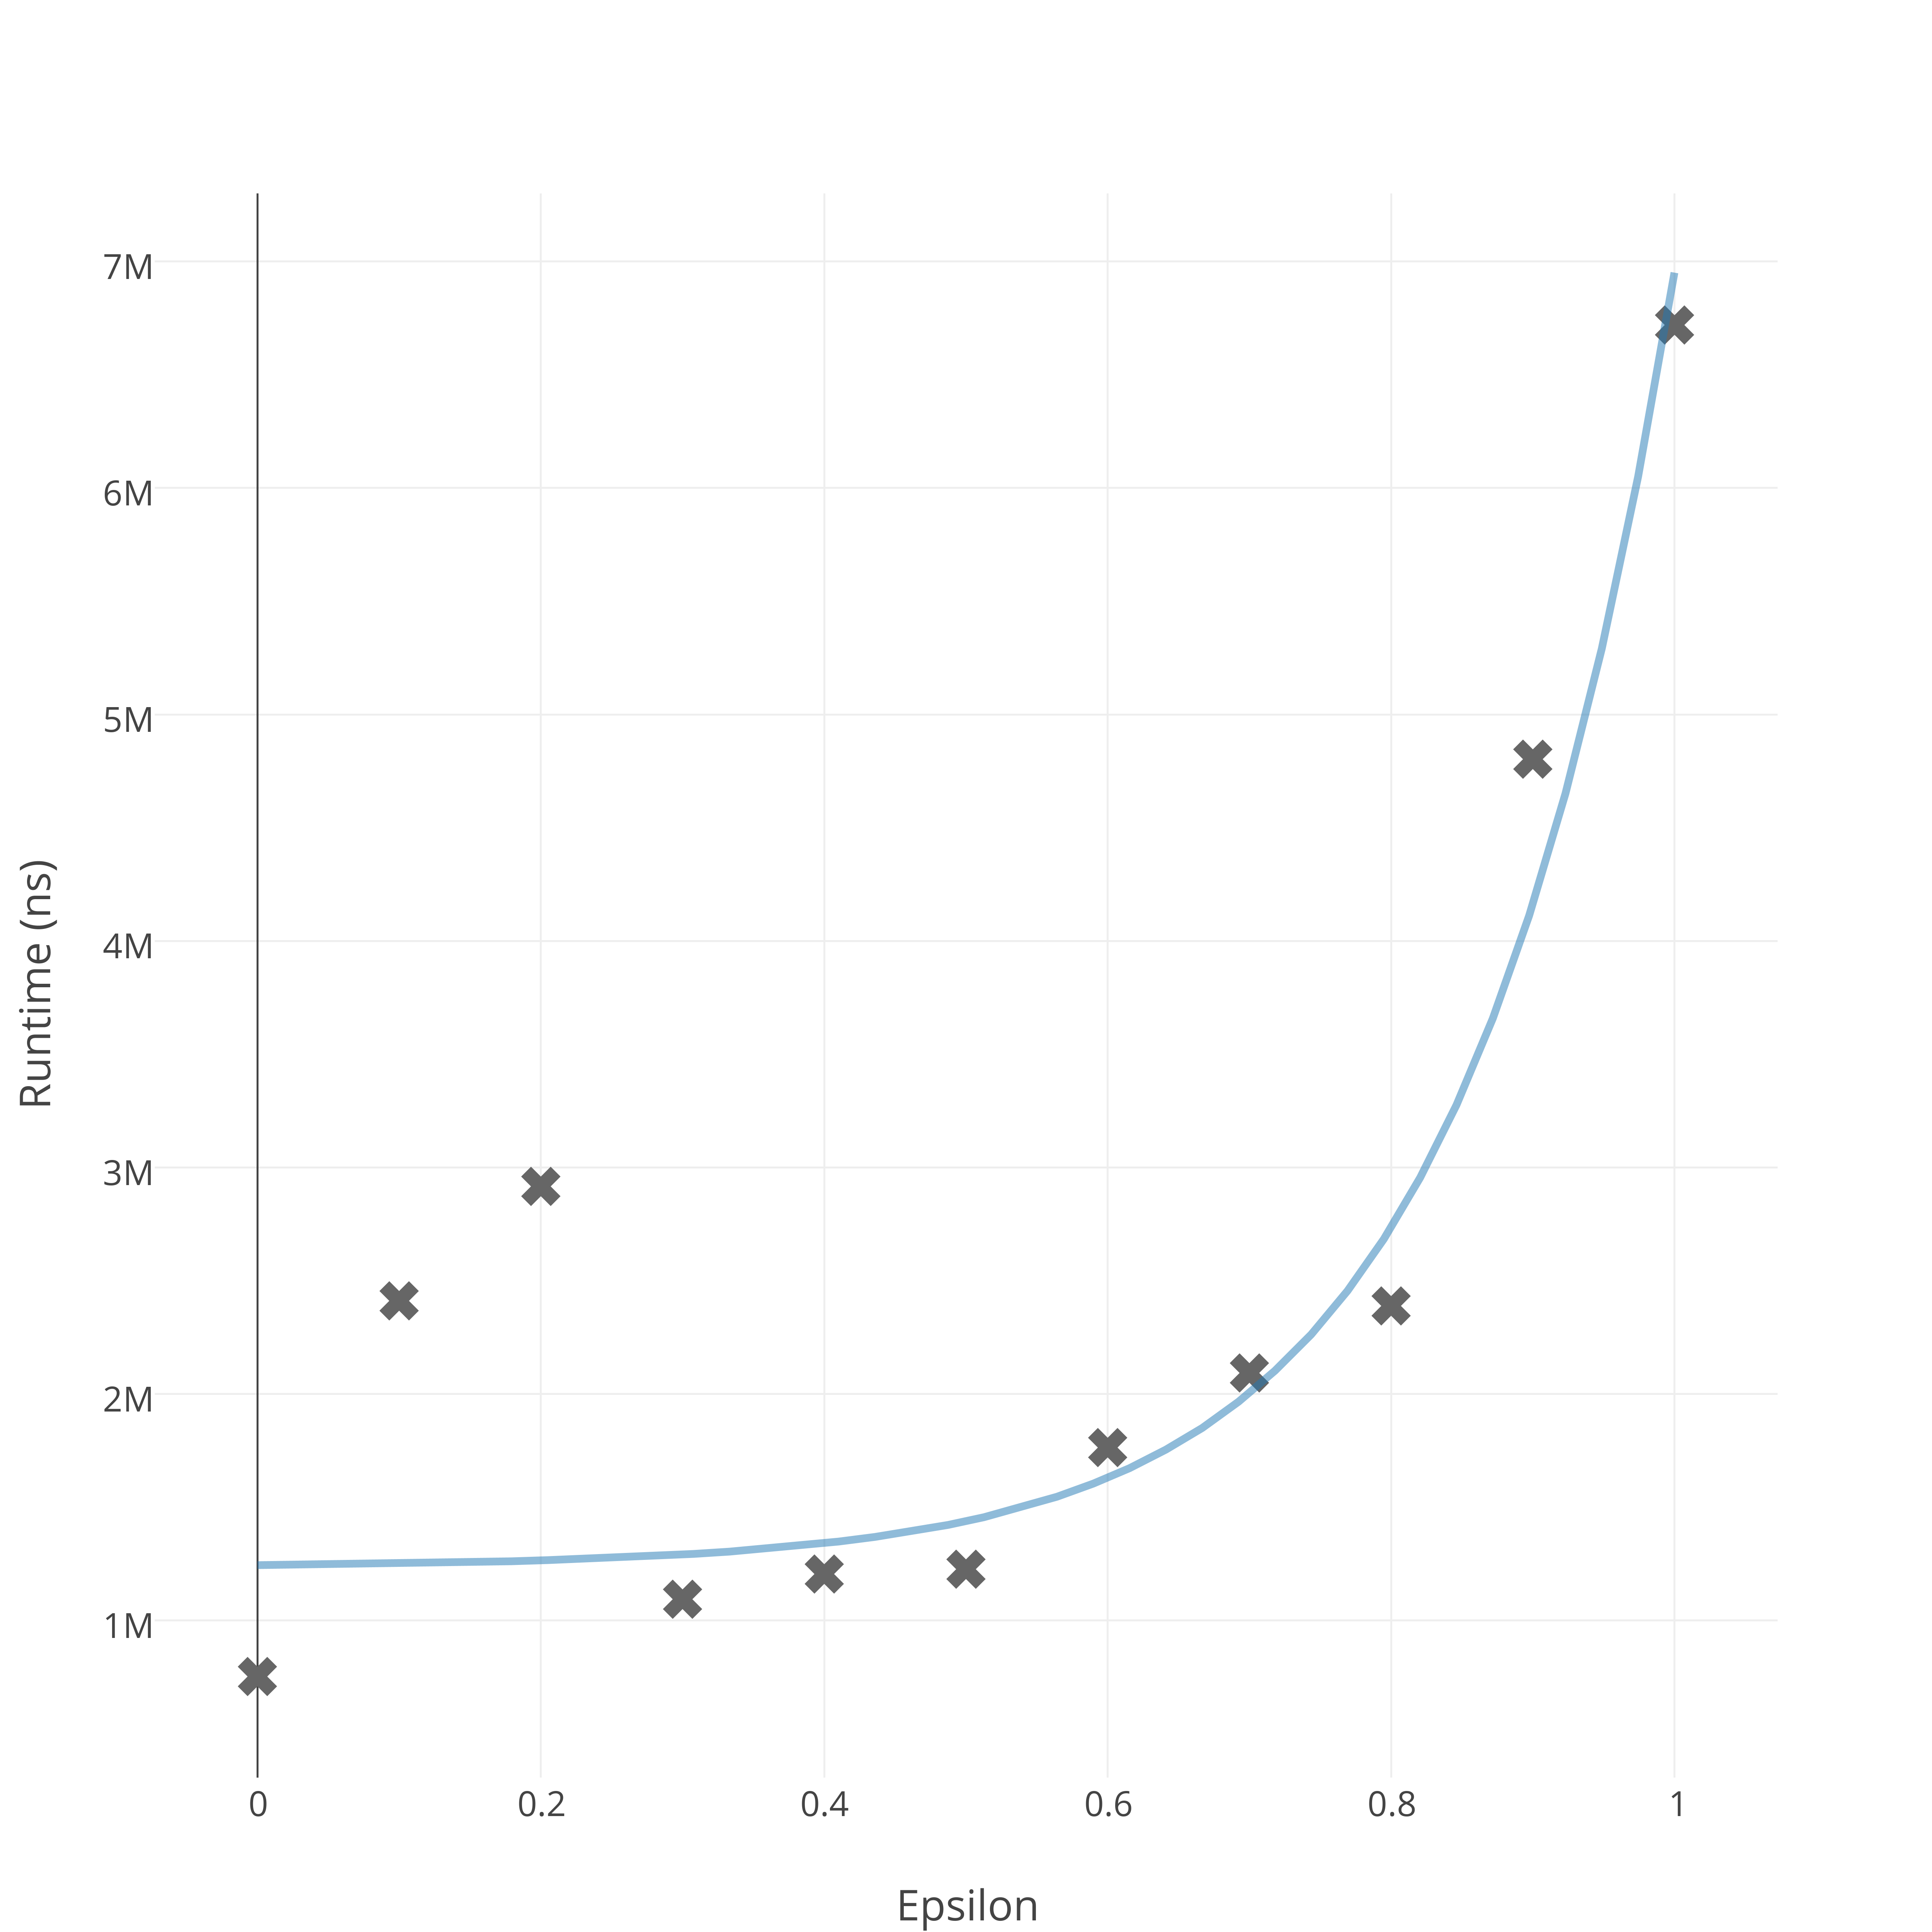
\includegraphics[width=.5\textwidth]{pics/runtimevsepsilon_medium}}{\centering\caption{$\epsilon$ vs runtime for the medium map for Q-learning. An exponential regression is superimposed on the graph.}\label{fig:qlruntimemedium}}
        \ffigbox{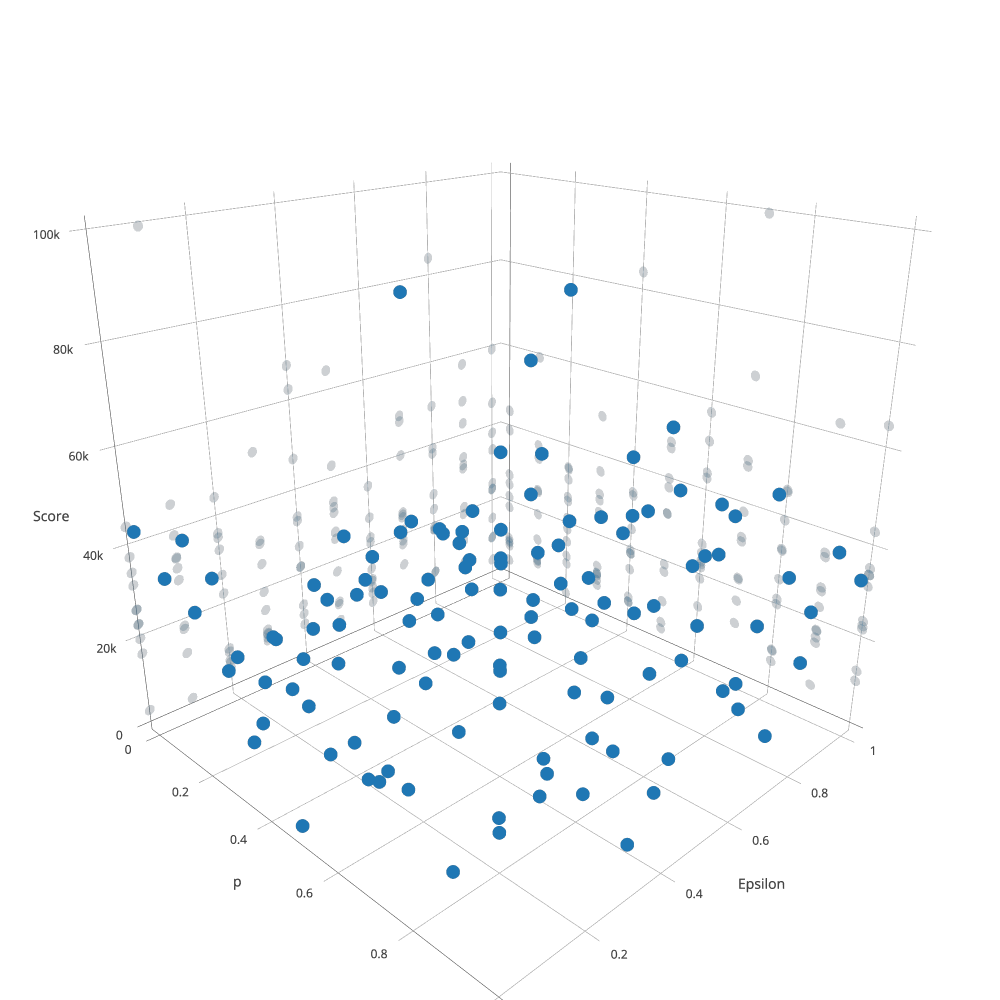
\includegraphics[width=.5\textwidth]{pics/QLearningBig}}{\centering\caption{Q-Learning scores for the big map over a space of $p$ and $\epsilon$ values, visualized as a 3D scatter plot.}\label{fig:qlscatterbig}}
    \end{floatrow}
\end{figure}